\textbf{Входные параметры:}
 
VHML\_ResultMatrix --- указатель на преобразуемый массив;
 
ProbabilityOfMutation --- вероятность мутации;
 
VHML\_N --- размер массива VHML\_ResultMatrix (число строк);
 
VHML\_M --- размер массива VHML\_ResultMatrix (число столбцов).

\textbf{Возвращаемое значение:} 

Отсутствует.

\textbf{Принцип работы:}
(на примере одной строки матрицы)

\begin{figure} [h]
  \center
  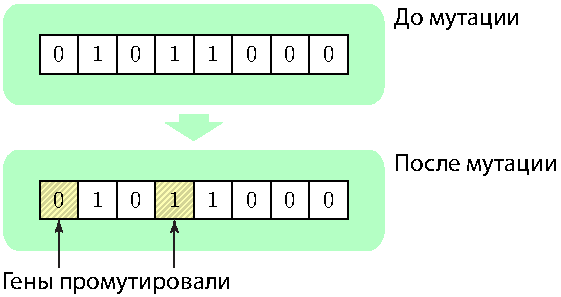
\includegraphics [scale=0.8] {HML_MutationBinaryMatrix_Sheme}
  \caption{Механизм работы мутации} 
  \label{img:HML_MutationBinaryMatrix_Sheme}  
\end{figure}
